% !TEX root = flow_head.tex
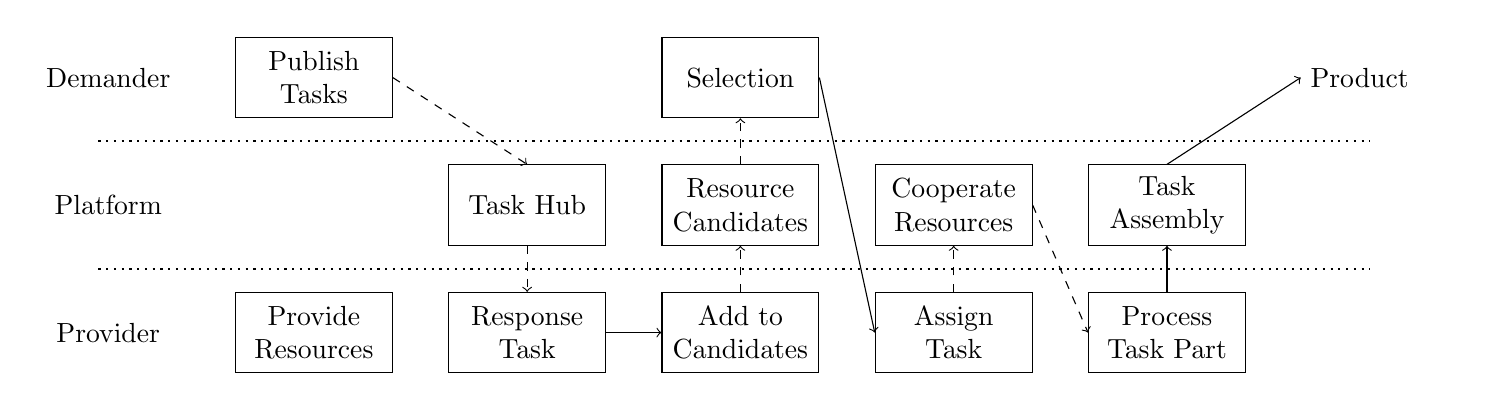
\begin{tikzpicture}[node distance=5mm and 5mm,
square/.style={
% The shape:
rectangle,
draw=black,
minimum size=2.9em,
text width=5em,
text centered
},
circle/.style={
rectangle,minimum size=1em,rounded corners=0.5em,
draw=black
}
]
\matrix[row sep=0.5em,column sep=2em] {
% First row:
\node (order) {Demander};& \node (task) [square]{Publish Tasks}; &  & \node (select) [square]{Selection}; & & &  \node (finish) {Product}; \\
\node (start1) {}; & & & & & & \node (stop1) {}; \\
\node (plt) {Platform} ; & &  \node (tb) [square] {Task Hub} ; & \node (candidate) [square] {Resource Candidates} ; & \node (coop) [square] {Cooperate Resources}; & \node (combine) [square] {Task Assembly};\\
\node (start2) {}; & & & & & & \node (stop2) {}; & \\
\node (provider) {Provider};  & \node (resource) [square]{Provide Resources}; & \node (response) [square] {Response Task}; & \node (add) [square]{Add to Candidates}; & \node (match) [square]{Assign Task}; & \node (process) [square] {Process Task Part};  &\\
};
\draw[dotted,thick] (start1.west) -- (stop1.east) (start2.west) -- (stop2.east);
\path[->,dashed] (task.east) edge (tb.north) (tb) edge (response) (add) edge (candidate) (candidate) edge (select) (match) edge (coop) (coop.east) edge (process.west);
\path[->] (response) edge (add) (select.east) edge (match.west) (process) edge (combine) (combine.north) edge (finish.west);
% \path (order) edge[->] (task) (task) edge[->] (match) (match) edge[->] (coord) (coord) edge[->] (process) (process) edge[->] (finish) (provider) edge[->] (resource) (resource) edge[->] (match);
\end{tikzpicture}